\documentclass[14pt, a4paper]{extreport}
\usepackage{susu}

\usepackage{subcaption}
\DeclareCaptionSubType*{figure}
\renewcommand\thesubfigure{\asbuk{subfigure})}
\DeclareCaptionLabelFormat{russian}{\MakeUppercase{#1~#2}}
\captionsetup[subfigure]{labelformat=russian, font=normalsize}

\begin{document}
	\firstpage
	\renewcommand\contentsname{ОГЛАВЛЕНИЕ}
	\tableofcontents
	\thispagestyle{empty}
\chapter* {ВВЕДЕНИЕ} 
	\addcontentsline{toc}{chapter}{ВВЕДЕНИЕ}
	Выпускная квалификационная работа является важным этапом в оценке знаний обучающегося. Данная работа призвана показать способности студента к самостоятельному поиску информации, исследованию, а также постановке и выполнению сложных задач. 
	
	Для ее успешного выполнения требуется использовать знания полученные в ходе всего обучения по выбранной студентом программе. При этом важно не только поставить цель и задачи, оценить их потенциал и актуальность, исследовать предметную область, и способы решения и по итогу выполнить их, но и правильно описать все описаное выше. Доступным, но при этом строгим и последовательным языком описать все описанные этапы выполнения выпускной кваллификационной работы.
	
	Пояснительная записка является подтверждением работы студента над поставленной задачей, показывает его умение правильно, четко и структурированно приподнести материал. Одним из важнейших частей данной работы является описание результатов разработанного алгоритма, а также выводы и заключения, подготовке речи и презентации.
	
	Оформлению даных пунктов и посвящена данная преддиплопная практика. В рамках практики планируется выполнить следующие задачи:
	\begin{enumerate}[label={\arabic*)}]
		\item оформление иллюстрационного материала, показывающего результаты работы;
		\item написание выводов по главе 2;
		\item написание выводов по главе 3;
		\item написание заключения к выпускной квалификационной работе;
		\item подготовка доклада и мультимедийной презентации.
	\end{enumerate} 
\chapter {ПОДГОТОВКА ИЛЛЮСТРАЦИОННОГО МАТЕРИАЛА}
	Первой частью работы на практике является подготовка иллюстрационный материал, показывающий результаты работы алгоритма и описывающий составленную тестовую выборку. Результаты проделанной работы представленны далее. Результаты проделанной работы представленны далее.
	
	В результате разработки алгоритмов подготовки данных, детекции трубы, а также непосредственно сегментации, был разработан программный модуль, реализующий сегментацию факела вредных выбросов. Для оценки точности работы разработанного модуля была сформирована и размечена тестовая выборка, состоящая из 300 последовательно записанных оптических и тепловых кадров, в также максимальных и минимальных температур с рассмотренной ранее дискретностью. Данная выборка была размечена вручную. Пример выборки представлен на рисунке~\ref{fig:test_vib}.
	
	\begin{figure}[h!]
		\vspace*{0.22cm}
%		\begin{subfigure}{.32\textwidth}
%			\centering
%			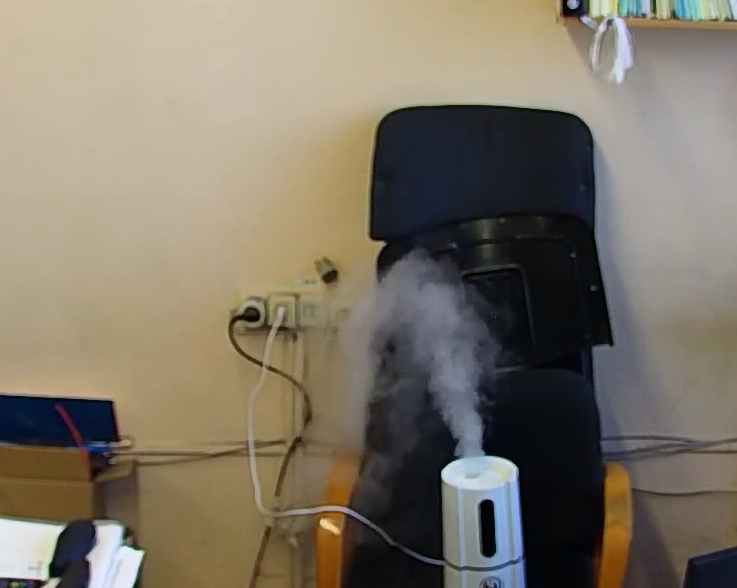
\includegraphics[width = \textwidth]{image/chapter_3/examples/img/151}
%			%			\caption{}
%		\end{subfigure}
%		\begin{subfigure}{.32\textwidth}
%			\centering
%			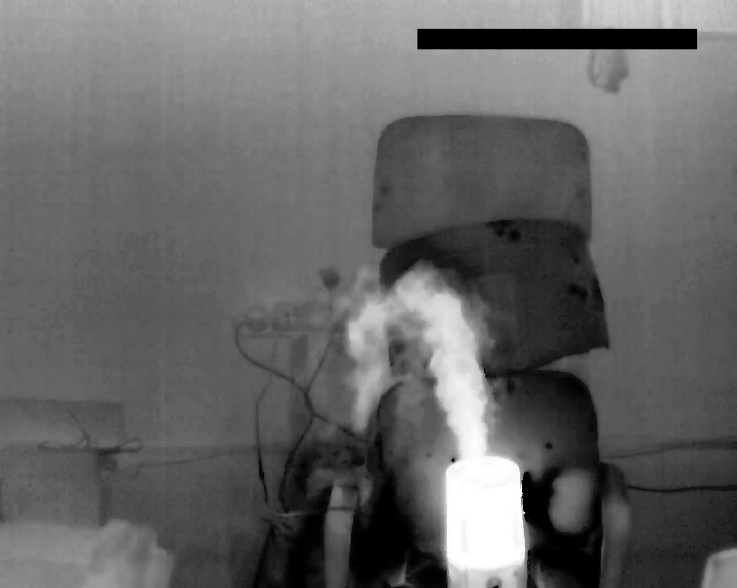
\includegraphics[width = \textwidth]{image/chapter_3/examples/tep/151}
%			%			\caption{}
%		\end{subfigure}
%		\begin{subfigure}{.32\textwidth}
%			\centering
%			
\includegraphics[width = \textwidth]{image/chapter_3/examples/mask_razmet/151}
%			%			\caption{}
%		\end{subfigure}
		\begin{subfigure}{.32\textwidth}
			\centering
			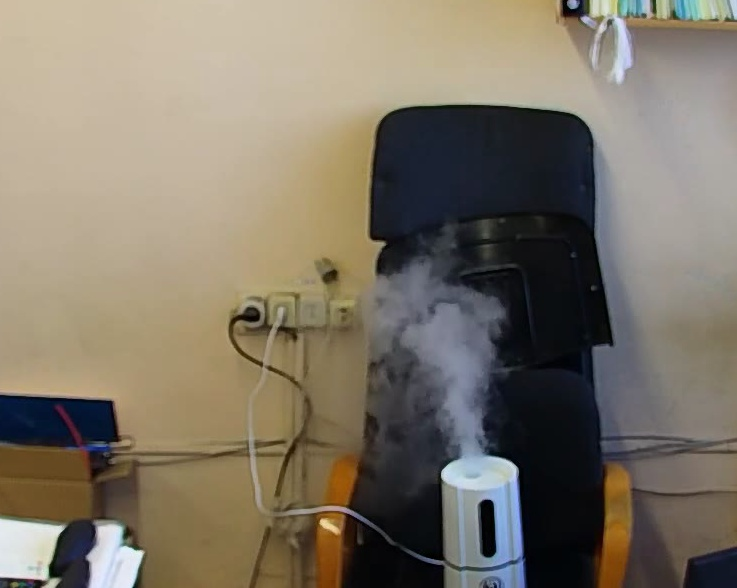
\includegraphics[width = \textwidth]{image/chapter_3/examples/img/185}
			%			\caption{}
		\end{subfigure}
		\begin{subfigure}{.32\textwidth}
			\centering
			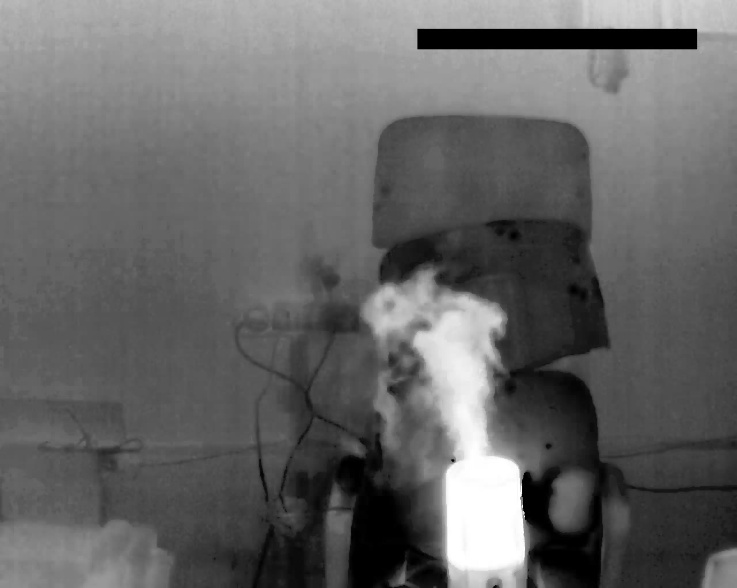
\includegraphics[width = \textwidth]{image/chapter_3/examples/tep/185}
			%			\caption{}
		\end{subfigure}
		\begin{subfigure}{.32\textwidth}
			\centering
			
\includegraphics[width = \textwidth]{image/chapter_3/examples/mask_razmet/185}
			%			\caption{}
		\end{subfigure}
		\begin{subfigure}{.32\textwidth}
			\centering
			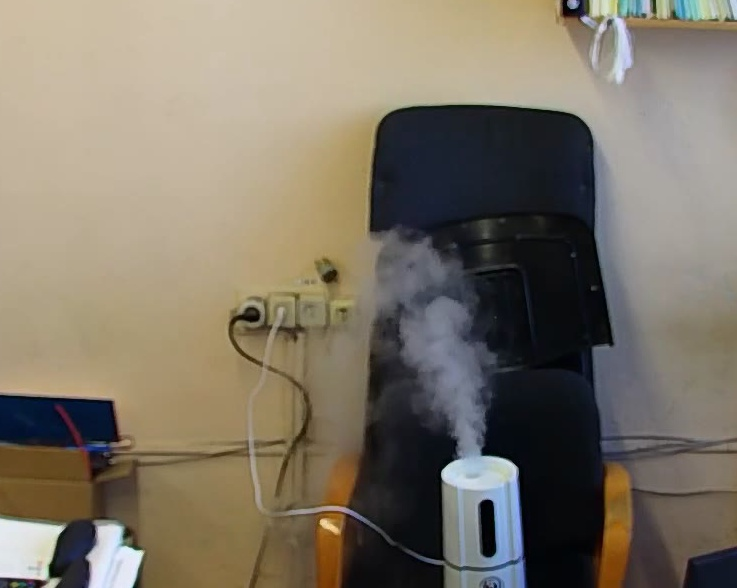
\includegraphics[width = \textwidth]{image/chapter_3/examples/img/159}
			\caption{}
		\end{subfigure}
		\hspace{0.1cm}
		\begin{subfigure}{.32\textwidth}
			\centering
			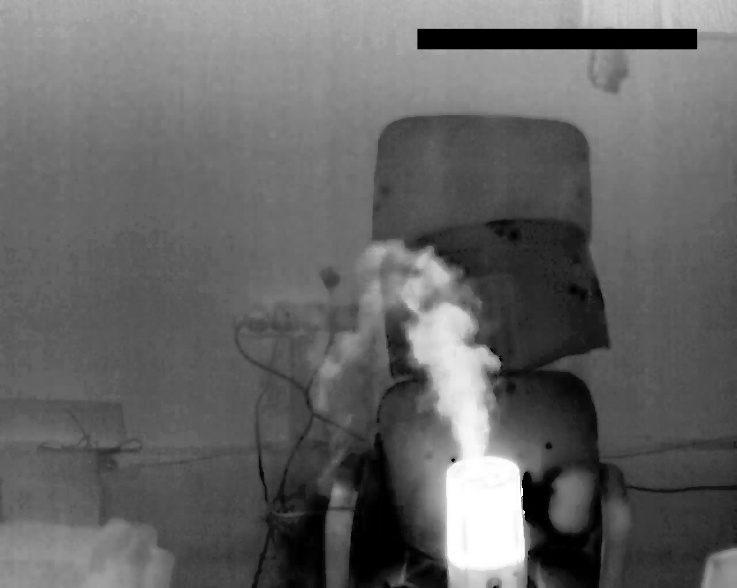
\includegraphics[width = \textwidth]{image/chapter_3/examples/tep/159}
			\caption{}
		\end{subfigure}
		\hspace{0.1cm}
		\begin{subfigure}{.32\textwidth}
			\centering
			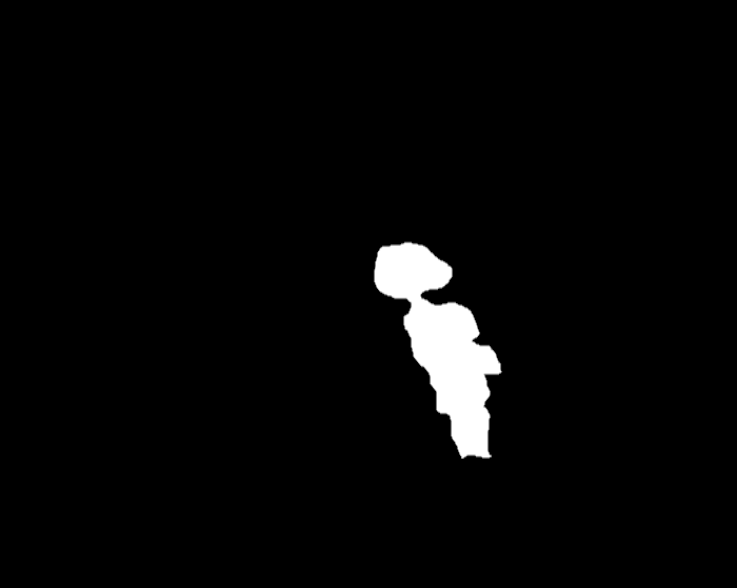
\includegraphics[width = \textwidth]{image/chapter_3/examples/mask_razmet/159}
			\caption{}
		\end{subfigure}
		\caption{Пример тестовой выборки: а) оригинальные оптические изображения; б) оригинальные тепловые изображения; в) маски}
		\label{fig:test_vib}
	\end{figure}
	
	Данная тестовая выборка состоит из записанных тепловизором выбранной модели данных. На данный момент данные являются синтетическими, и были получены в результате моделирования трубы и горячих выбросов из нее.
	
	Для тестирования и оценки реализованного программного комплекса, была проведена сегментация данной тестовой выборки (см.~рисунок~\ref{fig:test_segm}).
	\vspace*{-0.1cm}
	\begin{figure}[h!]
		\begin{subfigure}{.32\textwidth}
			\centering
			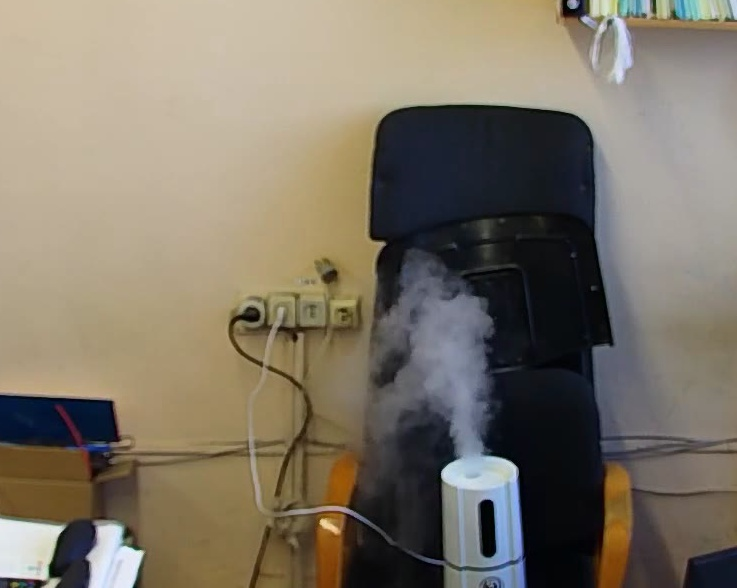
\includegraphics[width = \textwidth]{image/chapter_3/examples/img/206}
			%			\caption{}
		\end{subfigure}
		\begin{subfigure}{.32\textwidth}
			\centering
			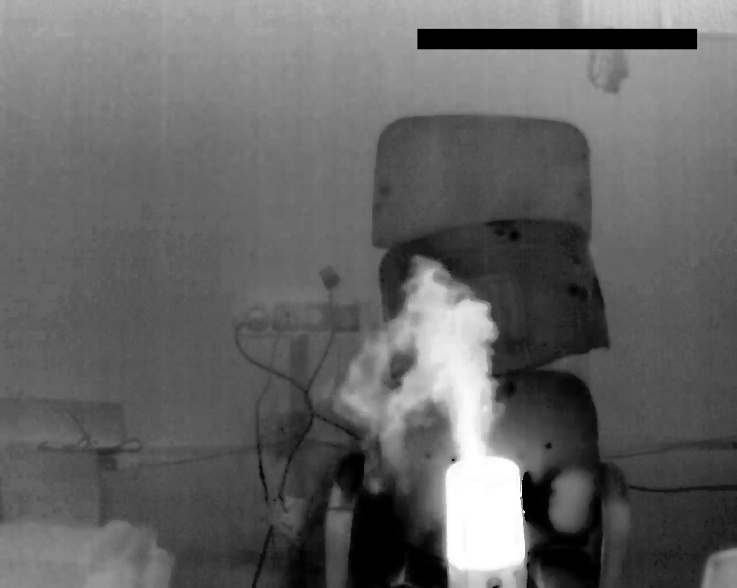
\includegraphics[width = \textwidth]{image/chapter_3/examples/tep/206}
			%			\caption{}
		\end{subfigure}
		\begin{subfigure}{.32\textwidth}
			\centering
			
\includegraphics[width = \textwidth]{image/chapter_3/examples/mask/206}
			%			\caption{}
		\end{subfigure}
		\begin{subfigure}{.32\textwidth}
			\centering
			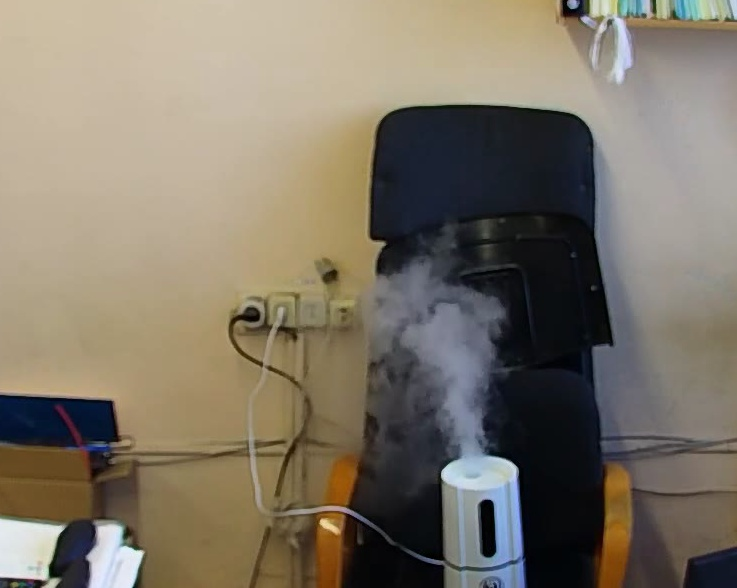
\includegraphics[width = \textwidth]{image/chapter_3/examples/img/185}
			%			\caption{}
		\end{subfigure}
		\begin{subfigure}{.32\textwidth}
			\centering
			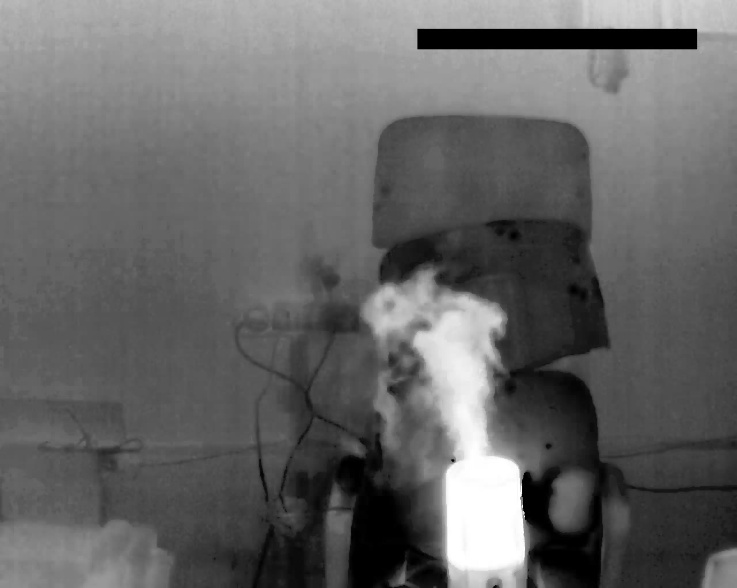
\includegraphics[width = \textwidth]{image/chapter_3/examples/tep/185}
			%			\caption{}
		\end{subfigure}
		\begin{subfigure}{.32\textwidth}
			\centering
			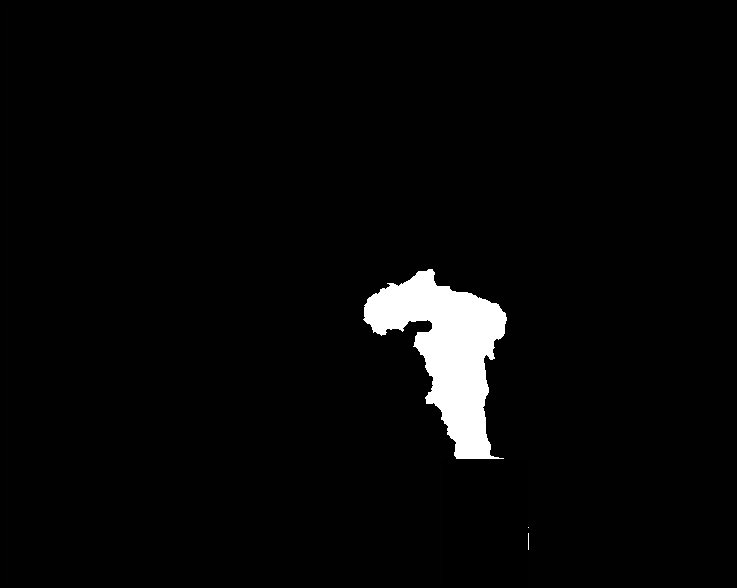
\includegraphics[width = \textwidth]{image/chapter_3/examples/mask/185}
			%			\caption{}
		\end{subfigure}
		\begin{subfigure}{.32\textwidth}
			\centering
			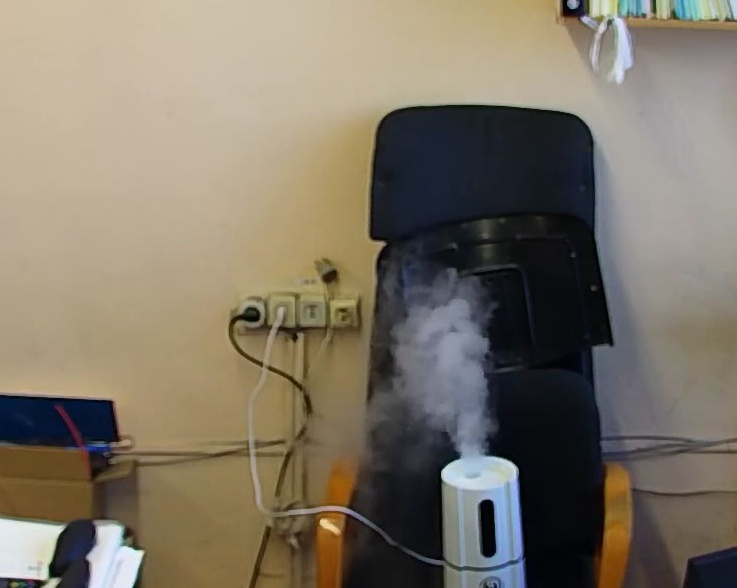
\includegraphics[width = \textwidth]{image/chapter_3/examples/img/214}
			%			\caption{}
		\end{subfigure}
		\begin{subfigure}{.32\textwidth}
			\centering
			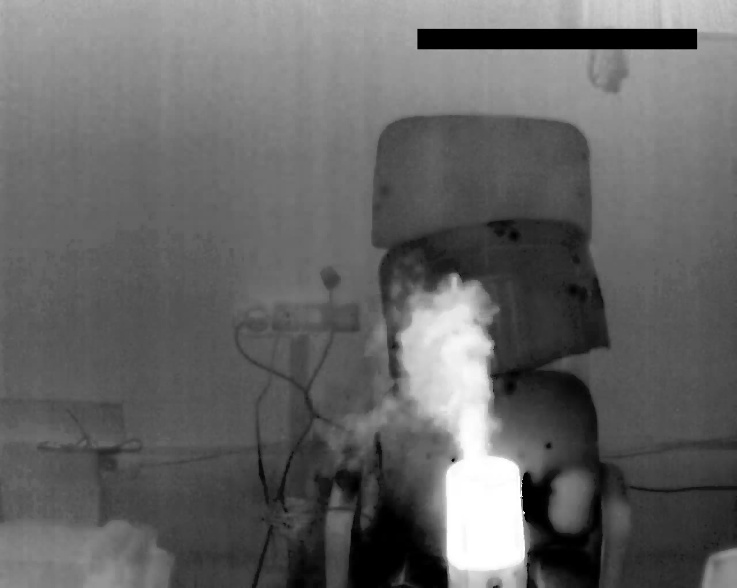
\includegraphics[width = \textwidth]{image/chapter_3/examples/tep/214}
			%			\caption{}
		\end{subfigure}
		\begin{subfigure}{.32\textwidth}
			\centering
			
\includegraphics[width = \textwidth]{image/chapter_3/examples/mask/214}
			%			\caption{}
		\end{subfigure}
		\begin{subfigure}{.32\textwidth}
			\centering
			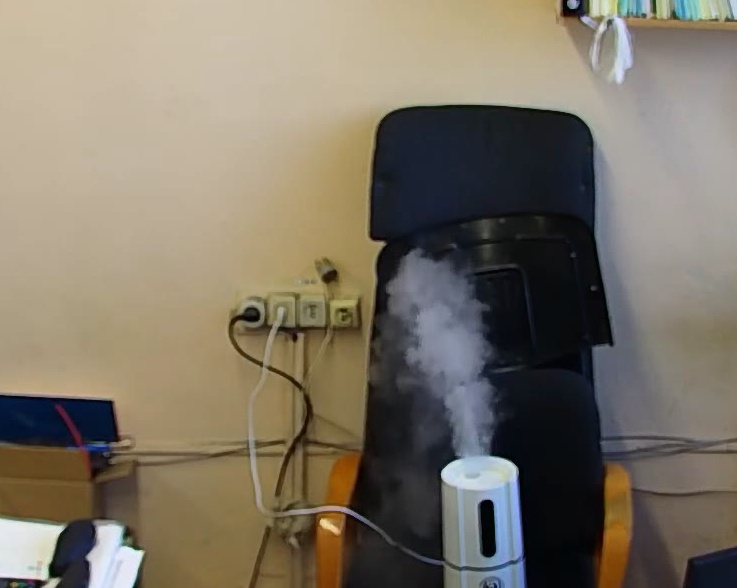
\includegraphics[width = \textwidth]{image/chapter_3/examples/img/240}
			\caption{}
		\end{subfigure}
		\hspace{0.1cm}
		\begin{subfigure}{.32\textwidth}
			\centering
			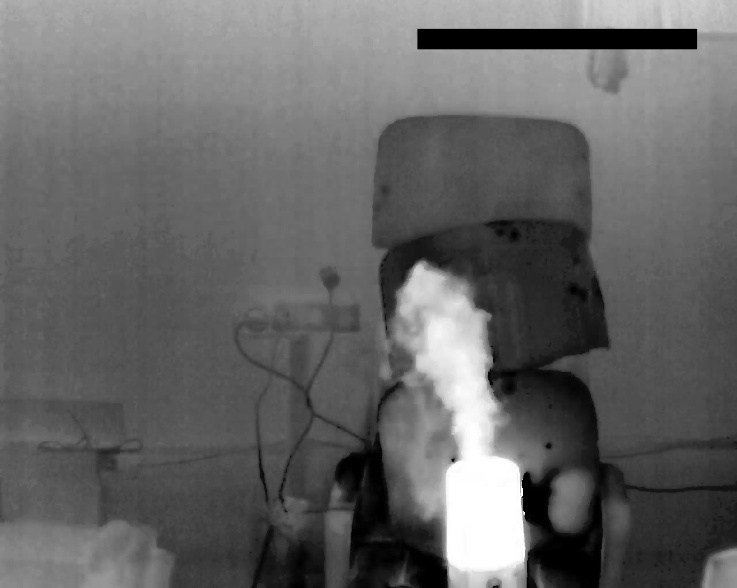
\includegraphics[width = \textwidth]{image/chapter_3/examples/tep/240}
			\caption{}
		\end{subfigure}
		\hspace{0.1cm}
		\begin{subfigure}{.32\textwidth}
			\centering
			
\includegraphics[width = \textwidth]{image/chapter_3/examples/mask/240}
			\caption{}
		\end{subfigure}
		\caption{Пример работы: а) оригинальные оптические изображения; б) оригинальные тепловые изображения; в) получившиеся маски}
		\label{fig:test_segm}
	\end{figure}
	
	Для оценки также необходимо ввести некоторую метрику. Метрика является некоторой функцией, отражающей то, на сколько результат работы того или иного алгоритма соответствует правильному. В случае бинарной сегментации (сегментации изображения на 2 класса) одной из наиболее подходящих метрик является метрика <<DICE>>, также известная как коэффициент Сёренсена-Дайса или F1-мера, является одним из показателей оценки сходства между двумя наборами данных. Она широко используется в задачах сегментации изображений [\ref{Rethinking dice loss for medical image segmentation}].
	
	DICE определяется как отношение двойного пересечения и суммы сегментированных объектов:
	\begin{equation}
		\textup{DICE} = \frac{2\textup{TP}}{2\textup{TP} + \textup{FP} + \textup{FN}},
		\label{eq:DiceLoss}
	\end{equation}
	где TP -- количество пикселей, которые были верно классифицированы как сегментированный объект (правильное предсказание сегмента);\\
	\hspace*{0.8cm}FP -- количество пикселей, которые были неправильно классифицированы как сегментированный объект (ложное предсказание сегмента);\\
	\hspace*{0.8cm}FN -- количество пикселей, которые были неправильно классифицированы как фон или другой класс (неправильное предсказание сегмента).
	
	Значение DICE находится в диапазоне от 0 до 1, где 1 означает идеальное совпадение двух сегментаций, а 0 указывает на полное несовпадение. DICE является компромиссом между полнотой (отношение TP к общему количеству истинных объектов) и точностью (отношение TP к общему количеству предсказанных объектов). Он позволяет оценивать как качество сегментации, так и ее объем.
	
	Далее по формуле~(\ref{eq:DiceLoss}) вычислим значение метрики точности на представленной выборке. Точность по всей тестовой выборке рассчитана как средняя точность по элементам выборки, она составила 0.861004. Далее на рисунке~\ref{fig:mask_dif} представлено сравнение элементов из множества предсказанных масок и реальных по соответствующим элементам тестовой выборки, а также разница, представляющая собой исключающее или по маскам (т.е. если на размеченной маске и на маске полученной в результате работы программы класс пикселя отличается, то на разнице яркость пикселя будет равна 255, иначе равна 0). Данный метод наглядно показывает работу выбранной метрики точности.
	
		
	\begin{figure}[h!]
		\begin{subfigure}{.32\textwidth}
			\centering
			
\includegraphics[width = \textwidth]{image/chapter_3/examples/mask_razmet/206}
			%			\caption{}
		\end{subfigure}
		\begin{subfigure}{.32\textwidth}
			\centering
			
\includegraphics[width = \textwidth]{image/chapter_3/examples/mask/206}
			%			\caption{}
		\end{subfigure}
		\begin{subfigure}{.32\textwidth}
			\centering
			
\includegraphics[width = \textwidth]{image/chapter_3/examples/mask_dif/206}
			%			\caption{}
		\end{subfigure}
		\begin{subfigure}{.32\textwidth}
			\centering
			
\includegraphics[width = \textwidth]{image/chapter_3/examples/mask_razmet/185}
			%			\caption{}
		\end{subfigure}
		\begin{subfigure}{.32\textwidth}
			\centering
			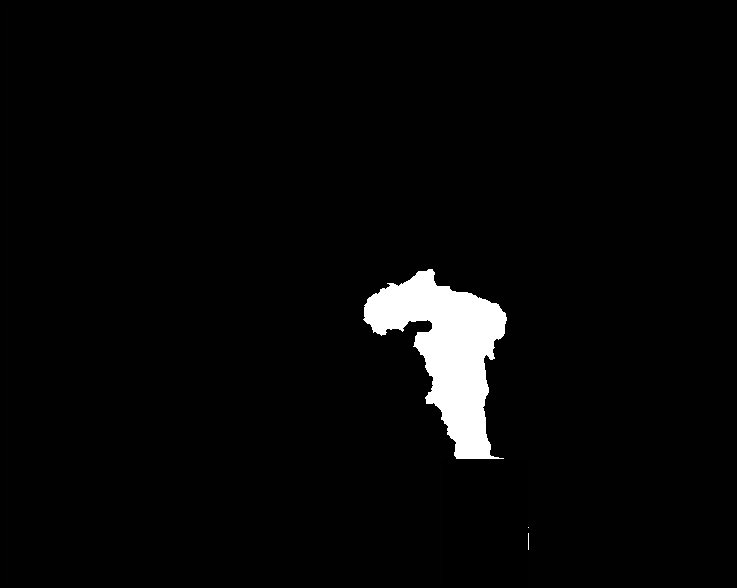
\includegraphics[width = \textwidth]{image/chapter_3/examples/mask/185}
			%			\caption{}
		\end{subfigure}
		\begin{subfigure}{.32\textwidth}
			\centering
			
\includegraphics[width = \textwidth]{image/chapter_3/examples/mask_dif/185}
			%			\caption{}
		\end{subfigure}
		\begin{subfigure}{.32\textwidth}
			\centering
			
\includegraphics[width = \textwidth]{image/chapter_3/examples/mask_razmet/214}
			%			\caption{}
		\end{subfigure}
		\begin{subfigure}{.32\textwidth}
			\centering
			
\includegraphics[width = \textwidth]{image/chapter_3/examples/mask/214}
			%			\caption{}
		\end{subfigure}
		\begin{subfigure}{.32\textwidth}
			\centering
			
\includegraphics[width = \textwidth]{image/chapter_3/examples/mask_dif/214}
			%			\caption{}
		\end{subfigure}
		\begin{subfigure}{.32\textwidth}
			\centering
			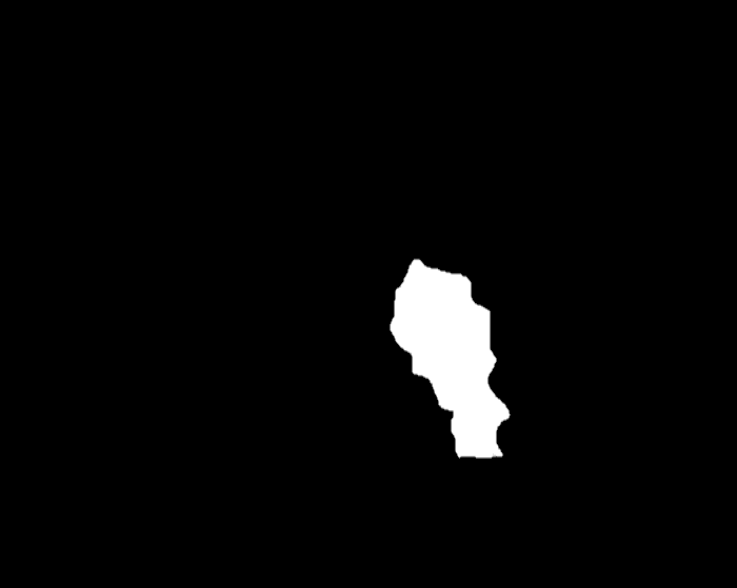
\includegraphics[width = \textwidth]{image/chapter_3/examples/mask_razmet/240}
			\caption{}
		\end{subfigure}
		\hspace{0.1cm}
		\begin{subfigure}{.32\textwidth}
			\centering
			
\includegraphics[width = \textwidth]{image/chapter_3/examples/mask/240}
			\caption{}
		\end{subfigure}
		\hspace{0.1cm}
		\begin{subfigure}{.32\textwidth}
			\centering
			
\includegraphics[width = \textwidth]{image/chapter_3/examples/mask_dif/240}
			\caption{}
		\end{subfigure}
		\caption{Сравнение масок: а) размеченная маска; б) результат работы алгоритма; в) исключающее или}
		\label{fig:mask_dif}
	\end{figure}
	
	Также для визуализации точности работы алгоритма ниже представлен график. На данном графике показана зависимость точности от номера кадра, с помощью которой можно получить представление о разбросе точности работы алгоритма(см.~рисунок~\ref{fig:accuracy_itog_plot}). В результате можно сказать о достаточно высокой точности работы алгоритма, а также о малом разбросе.
	\begin{figure}[h!]
		\centering
		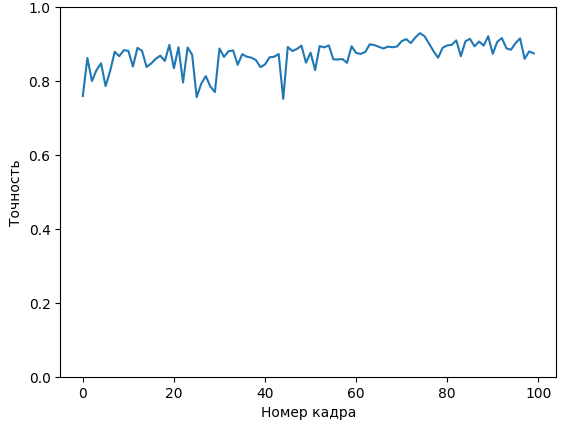
\includegraphics[width = 0.9\textwidth]{image/chapter_3/accuracy_itog_plot}	
		\caption{Пример сопоставления ключевых точек}
		\label{fig:accuracy_itog_plot}
	\end{figure}

	Помимо этого были подготовленны презентация и доклад. Текст доклада можно увидеть в приложении 1, подготовленую презентацию в прилоджении 2.

\chapter {ОФОРМЛЕНИЕ ВЫВОДОВ К РАБОТЕ}

	Также были написаны выводы к главам 2 и 3, а также заключение ко всей работе. Ниже представлен вывод по главе 2.
	
	Данная работа посвящена исследованию задачи сегментации факела выбросов с использованием данных тепло-видео системы наблюдения. Во второй главе дается строгая математическая постановка задачи.
	
	В данной главе приведен подробный алгоритм подготовки данных. Описаны математические модели работы с тепловизором, преобразования цветовой карты и наложения матрицы температур, а также используемых для этого вспомогательных алгоритмов и моделей класического машинного обучения.
	
	Для преобразования цветов была использованна непараметрическая модель <<k ближайших соседей>>. Используемая модель реализована с помощью структуры данных <<k--мерное дерево>>.
	
	Описана также математическая модель алгоритма детекции трубы, построенная на методе инвариантного преобразования особенностей, их сопоставления с помощью алгоритма <<k ближайших соседей>>, а также востановления трубы с помощью алгоритма <<RanSaC>>. Данный этап является одним из ключевых этапов сегментации.
	
	Подробно рассмотрен метод сегментации водоразделами. Данный метод отличается высокой скоростью работы, а также достаточно высокой точностью при работе с зашумленными изображениями. Подробное описание метода представленно в соответствующей части главы. Для решения поставленой задачи было решено использовать модифицированную версию алгоритма, включающую спользование маркеров.
	
	Также был оформлен вывод к главе 3. Он представлен ниже.
	
	В данной работе исследуется решение задачи сегментации факела выбросов с использованием данных тепло-видео систем наблюдения. В третьей главе приводится разработанные алгоритмы, согласно определенной ранее математической модели, а также результаты их работы, оценка точности.
	
	Приведены алгоритмы рассмотренных ранее этапов подготовки данных с результатами работы. Для преобразования цветовой карты был разработан алгоритм на базе модели <<k ближайших соседей>>. Были приведены результаты работы, а также оценена точность в зависимости от степени сжатия. Оценка точности показала, что разработанный алгоритм работает достаточно точно даже при самых высоких уровнях сжатия, показывая точность выше 98\%.
	
	Был разработан алгоритм детекции трубы, использующий метод инвариантного преобразования особенностей для получения особых точек и алгоритм <<k ближайших соседей>> для их сопоставления. Данная часть работы показала свою необходимость для дальнейшего получения маркеров для алгоритма сегментации.
	
	В качестве алгоритма сегментации был разработан и реализован алгоритм сегментации водоразделами. Данный алгоритм является устойчивым к шуму, так как использует заранее подготовленные маркеры. В качестве данных маркеров было решено использовать трубу, как самый горячий объект, а также самую холодную область на изображении. Были приведены результаты работы алгоритма на подготовленной тестовой выборке. Также на этой выборке была посчитана точность алгоритма по метрике <<DICE>>, которая составила 86,2\%. помимо количественной оценки точности был также приведен график точности в зависимости от кадра видео, который показывает разброс точности работы алгоритма, а также наглядные иллюстрации с разницей между заранее подготовленными масками и результатами работы алгоритма. Еще одним преимуществом работы алгоритма является его быстродействие, так как время, затрачиваемое на каждый этап алгоритма, линейно зависит от размера подаваемого изображения, что в рассматриваемой задаче является оптимальным временем работы.
	
	Также было написано заключение ко всей работе. Оно представлено ниже.
	
	Целью данной работы являлась разработка алгоритма сегментации факела выбросов с использованием тепло-видео систем с реализацией в виде программного модуля, как ответ на проблему загрязнения окружающей среды вредными выбросами предприятий. В ходе работы была сформулирована задача бинарной сегментации пары из изображения и матрицы температур, а также рассмотрены современные способы контроля за вредными выбросами и способы применения тепло-видео систем наблюдения. Для решения задачи были выбраны классические методы сегментации, опирающиеся на высокую температуру выбросов.
	
	Алгоритм сегментации был разделен на два этапа. Первым этапом является подготовка данных. Решение это подзадачи оказалось нетривиальным и потребовало использования методов машинного обучения, а конкретно алгоритма <<k ближайших соседей>>. Для оценки данных методов была сформулирована метрика точности и была посчитана точность. Результаты показали высокую точность, даже при сильном сжатии изображения.
	
	Вторым этапом является непосредственно сегментация. Она в свою очередь делится на этап детекции трубы, а также сегментацию факела выбросов. Для решения задачи детекции трубы был использован инвариантного преобразования особенностей и алгоритм <<k ближайших соседей>>. Детекция трубы является важным этапом сегментации, так как позволяет получить маркеры для дальнейшей сегментации. Одним из преимуществ данного подхода является высокое быстродействие.
	
	Для сегментации факела выбросов был использован метод сегментации водоразделами, с применением маркеров. Данный метод был протестирован на тестовой выборке, представляющей из себя тепловое и оптическое видео длинной в 100 кадров, размеченные в ручную. На данной тестовой выборке алгоритм был протестирован с использование метрики точности <<DICE>>. Была получена точность 86,2\%. Также были продемонстрированы график точности и иллюстрации разницы между подготовленными и посчитанными алгоритмом масками. на основании всех этих данных можно сделать вывод о достаточно высокой точности алгоритма. Также были сделаны выводы о его высоком быстродействии.
	
	Таким образом цели работы были достигнуты, а поставленная\linebreak задача -- решена. Представленное в работе решение может быть использовано для сегментации выбросов для дальнейшего получения информации в рамках проекта <<Экомонитор>>. В виду большого количества информации потенциально скрытого в тепловых матрицах, такого как возможная зависимость между объемом выбросов и их температурой, дальнейшими целями для развития работы может стать получение физических характеристик факела выбросов.


\chapter* {ЗАКЛЮЧЕНИЕ} 
	\addcontentsline{toc}{chapter}{ЗАКЛЮЧЕНИЕ}
	Данная преддипломная практика посвящена подготовке иллюстрационого материала, написанию выводов и заключения по проделанной работе. В ее рамках были подготовленны иллюстрационные материалы к работе алгоритма и подготовленой тестовой выборке, описана метрика точности и проведена оценка точности разработанного алгоритма.
	
	Были сформулированы и написаны выводы к главам 2 и 3. Также было написано заключение к выпускной кваллификационной работе.
	
	Помимо этого также были подготовлены доклад и мультимедийная презентация для защиты выпускной кваллификационной работы. Текст доклада, а также подготовленная презентация приведены в приложениях. 
	
	В результате преддипломной практики были выполнены все поставленные, в следствии чего была полностью подготовлена пояснительная записка к выпускной кваллификацинной работе, а также мультимедийная презентация и доклад.
\chapter* {БИБЛИОГРАФИЧЕСКИЙ СПИСОК} 
	\addcontentsline{toc}{chapter}{БИБЛИОГРАФИЧЕСКИЙ СПИСОК}
	\begin{sortedlist_eng}
				\sortitem{\vspace{1cm}\textbf{Zhao,~R.} Rethinking dice loss for medical image segmentation / R.~Zhao, B.~Qian, X.~Zhang // 2020 IEEE International Conference on Data Mining (ICDM). -- 2020. -- P.~851--860.}{Rethinking dice loss for medical image segmentation}{ZhaoQianZhangRethinkingdiceloss}
				\sortitem{\textbf{Beucher,~S} The watershed transformation applied to image\linebreak segmentation / K.~V.~Lalitha, R.~Amrutha, S.~Michahial // Scanning\linebreak Microscopy. -- 1992. -- V.~1992, №~6. -- P.~299--314.}{Implementation of watershed segmentation}{Beucher}
	\end{sortedlist_eng}
\chapter* {ПРИЛОЖЕНИЕ 1}
	\addcontentsline{toc}{chapter}{ПРИЛОЖЕНИЕ 1 Текст доклада}
	\vspace{-0.5cm}
	\hspace{5.1cm} Текст доклада
	
	Слайд 1. Здравствуйте уважаемые председатель и члены государствунной экзаменационной комиссии. Тема моей выпускной кваллификационной работы -- Решение задачи сегментации
	факела выбросов на основе данных тепло-видео системы наблюдения. Сегодня очень важен вопрос загрязнения окружающей среды и сегментация факела выбросов поможет эфективней контролировать выбросы предприятий.
	
	Слайд 2. Целью данной работы является разработка алгоритма сегментации факела выбросов с использованием тепло-видео систем. Задачи представлены на слайде.
	
	Слайд 3. Мной были исследованы современные методы контроля вредных выбросов. Их классификация представленна на слайде. Было выявлено, что инструментальный метод является трудным в исполнении и дорогим, тогда как расчетный метод -- недостаточно точным. Одним из решений этой проблемы является сегментация факела выбросов.
	
	Слайд 4. Для сегментации выбросов можно использовать тепловизоры, так как выбросы имеют высокую температуру, что обеспесивает их лучшую видимость на тепловых снимках, в отличии от оптических. Также они дешевле чем газоанализаторы. 
	
	Слайд 5. Постановка задачи сегментации факела выбросов звучит следующим образом: X -- пространство пар изображений и соответствующих им матрц температур. Z -- пространство масок соответствующей разменрности где каждый пиксель отражает вероятность принадлежности к факелу. Необходимо восстановить функцию (1).
	
	Слайд 6. Задача сегментации факела выбросов делится на 3 основных этапа. Это подготовка даных, Детекция трубы, Сегментация факела.
	
	Слайд 7. Оссобенностью использованного тепловизора является вывод матрицы температур в формате цветного 3-х канального  сжатого изображения, поэтому требуется переход к одноканальному изображению в оттенках серого, где черный соответствует холодному, белый -- горячему.
	
	Слайд 8. Поэтому необходимо классифицировать цвета по 256 классам. Из за сжатия и искажения цветов было решено использовать модель классификации <<k ближайших соседей>>, которая для каждого цвета находит ближайший цвет из тестовой выборки и классифицирует его классом этого цвета.
	
	Слайд 9. Здесь представленна схема этого алгоритма. Ключевой момент -- подготовка классификатора цветов, для этого обучаем модель на 256 оттенках серого и классифицируем все RGB пространство. 
	
	Слайд 10. Для анализа точности алгоритма была сформулированна следующая метрика точности, соответсвующая среднему евклидовому расстоянию между интенсивностью пикселей, которую вы можете увидеть на слайде. 
	
	Слайд 11. Здесь видно как меняется точность в зависимости от степени сжатия изображения.
	
	Слайд 12. Здесь показан пример результата подготовки данных до подготовки и после, теловизионное изображение преобразовано к одноканальному формату, оба изображения имеют один размер.
	
	Слайд 13. 2 этап -- задача детекции трубы. Зачастую температура трубы выше чем температуры выбросов, как следствие алгоритмы сегментации основанные на температуре сегментируют и трубу. Поэтому нам необходима детекция трубы заданной на образце
	
	Алгоритм делится на три шага: первый шаг получение ключевых точек на изображении образце и на входном изображении. Второй шаг -- классификация ключевых точек по точкам на изображении образце. третий шаг восстановление координат прямоугольника с трубой. 
	
	Слайд 14. Шаги 1 и 3 представленны в виде схем. Получаем пирамиду изображений в разной степени размытых фильтром гаусса, после каждую точку проверяем на локальный экстремум в пирамиде и контрастность, и добавляем дескриптор в случае успеха.
	для востановления координат мы некоторое количесво раз выбираем 2 случайные ключевые точки, восстанавливаем по ним прямоугольник и обновляем лучшый результат.
	
	Слайд 15. 3 этап -- сегментация методом водораздела, он был выбран потому что матрица температур является черно белым изображеним с низкой контрастностью, а также потому что данный алгоритм позволяет работать с маркерами. Простыми словами можно описать алгоритм следующим образом: градиент функции представляется в виде поверхности, в маркерах проделываются отверстия, и начинается затопление этой поверхности. В месте соединения воды появляется водораздел являющийся границей классов сегментации.
	
	Слайд 16. Тут можно увидеть алгоритм сегментации. Находятся маркеры, классу выбросов соответствует самая <<горячая точка трубы>>, классу не выбросов соответствует самая холодная точка изображения. Вычисляется градиент, преобразовывается с помощью маркеров и делится на секции уровней. Для каждой секции уровня вычисляется новая зона влияния каждого маркера. После из полученной маски исключается\linebreak прямоугольник с трубой
	
	Слайд 17. Для тестирования алгоритма была сформирована синтетическая тестовая выборка и на рисунке 12 можно увидеть пример работы алгоритма сегментации.
	
	Слайд 18. Данная тестовая выборка была в ручную размечена и на рисунке 15 представлеенна визуализация разницы масок, размеченых вручную и масок полученных с помощью алгоритма. 
	
	Слайд 19. Для оценки точности решено было использовать коэффициент Серенсена - Дайса, вычисляемый по формуле 3. Здесь TP FP и FN -- площади соответствующих сегментов. Метрика позволяет оценивать как качество сегментации, так и ее объем. Получившаяся точность -- 86,2\%
	
	Слайд 20. В ходе работы был разработан алгоритм сегментации факела выбросов, исползующий данные тепло-видео систем наблюдения. Данная работа выполнена в рамках проекта <<Экомонитор>> института естественных и точных наук.
	
	Была разработана математическая модель алгоритмов подготовки данных, детекции трубы и сегментации факела выбросов методом водораздела. Данные алгоритмы были разработаны, реализованы и протестированы. Таким образом цель работы достигнута, а все поставленные задачи решены
	
	Слайд 21. Спасибо за внимание, готов ответить на ваши вопросы
	
	
\chapter* {ПРИЛОЖЕНИЕ 2}
	\renewcommand{\thefigure}{П2.\arabic{figure}}
	\addcontentsline{toc}{chapter}{ПРИЛОЖЕНИЕ 2 Презентация}
	\vspace{-0.5cm}
	\hspace{5.4cm} Презентация
	\begin{figure}[h!]
		\centering
		
\includegraphics[width = 0.8\textwidth]{image/процентовка1_page-0001}	
		\caption{Страница презентации 1}
	\end{figure}
	\begin{figure}[h!]
		\centering
		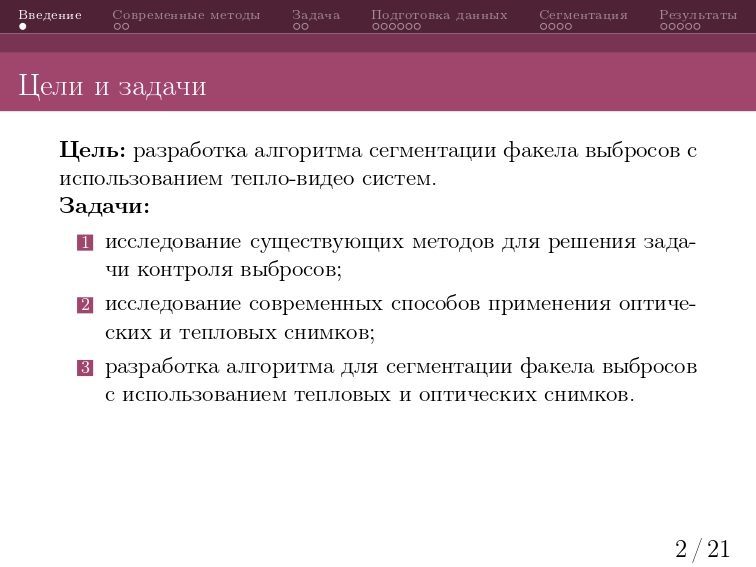
\includegraphics[width = 0.8\textwidth]{image/процентовка1_page-0002}	
		\caption{Страница презентации 2}
	\end{figure}
	\begin{figure}[h!]
		\centering
		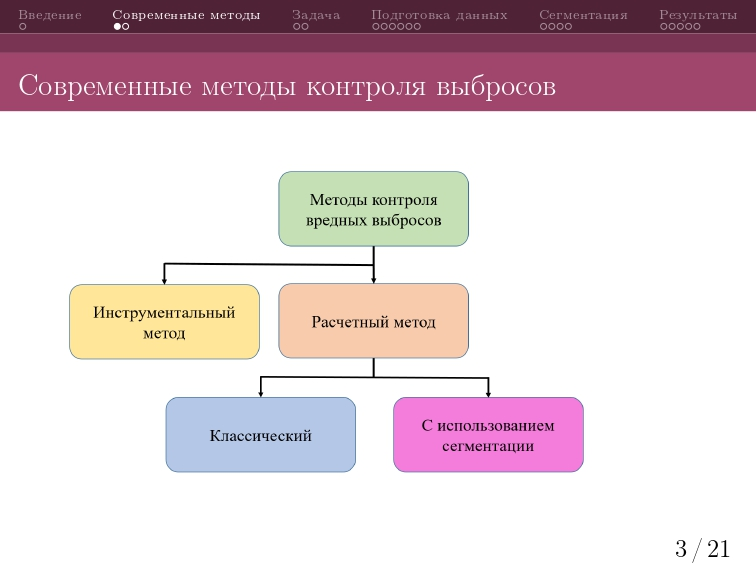
\includegraphics[width = 0.8\textwidth]{image/процентовка1_page-0003}	
		\caption{Страница презентации 3}
	\end{figure}
	\begin{figure}[h!]
		\centering
		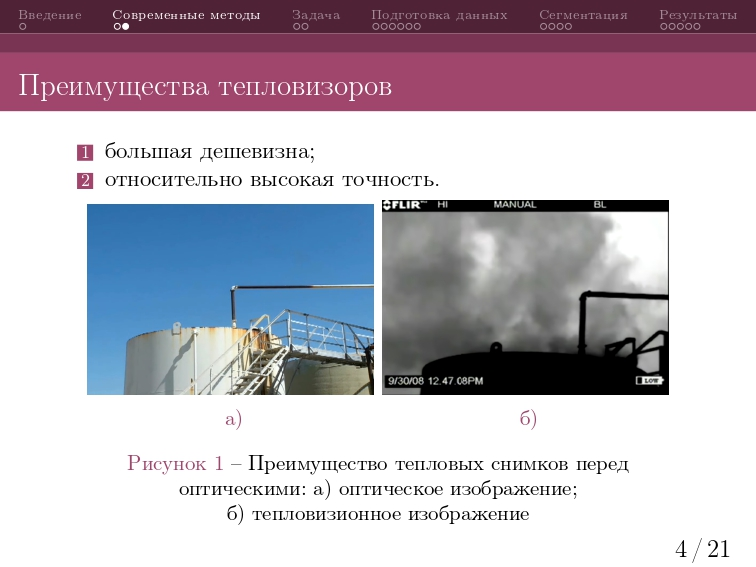
\includegraphics[width = 0.8\textwidth]{image/процентовка1_page-0004}	
		\caption{Страница презентации 4}
	\end{figure}
	\begin{figure}[h!]
		\centering
		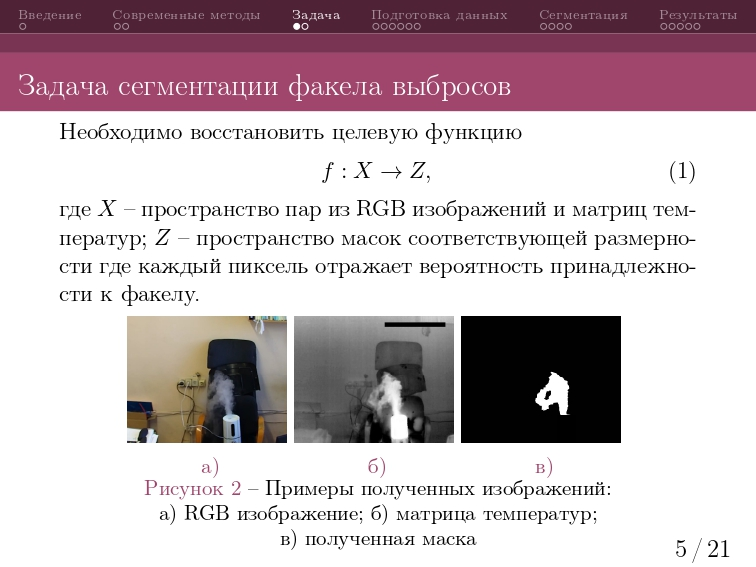
\includegraphics[width = 0.8\textwidth]{image/процентовка1_page-0005}	
		\caption{Страница презентации 5}
	\end{figure}
	\begin{figure}[h!]
		\centering
		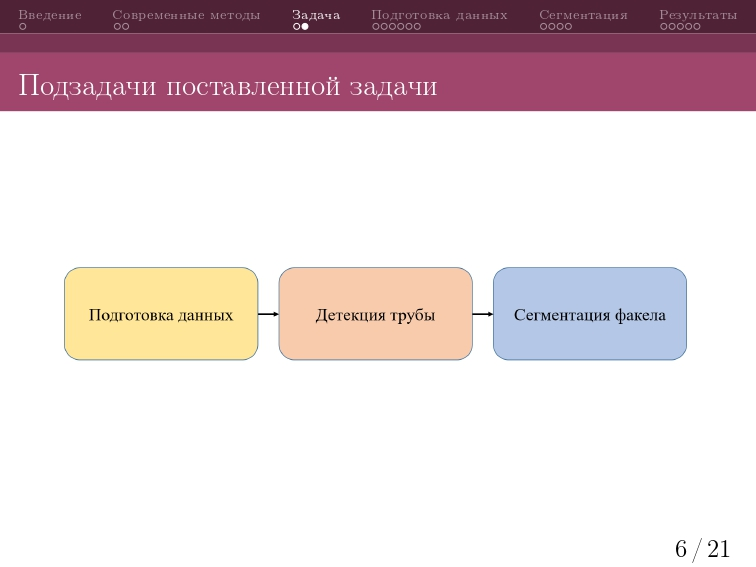
\includegraphics[width = 0.8\textwidth]{image/процентовка1_page-0006}	
		\caption{Страница презентации 6}
	\end{figure}
	\begin{figure}[h!]
		\centering
		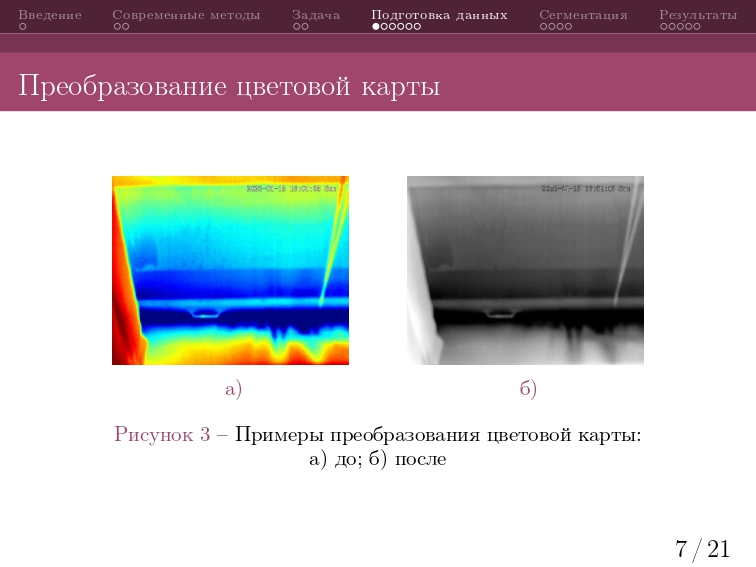
\includegraphics[width = 0.8\textwidth]{image/процентовка1_page-0007}	
		\caption{Страница презентации 7}
	\end{figure}
	\begin{figure}[h!]
		\centering
		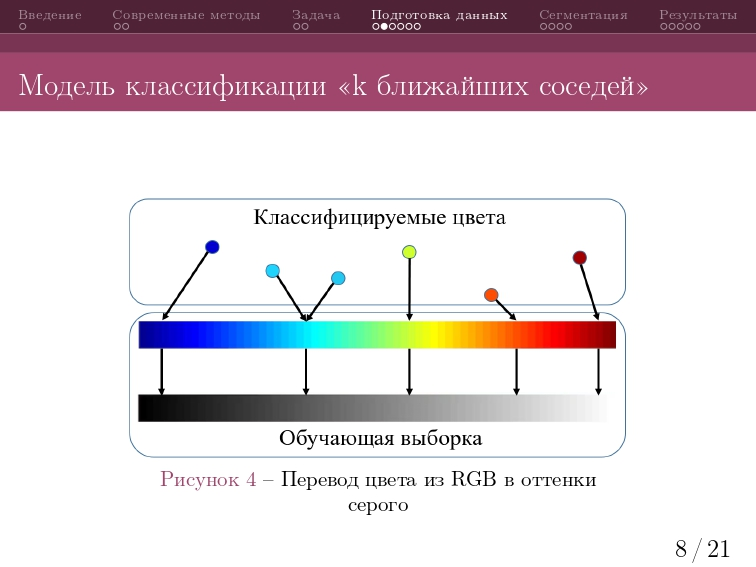
\includegraphics[width = 0.8\textwidth]{image/процентовка1_page-0008}	
		\caption{Страница презентации 8}
	\end{figure}
	\begin{figure}[h!]
		\centering
		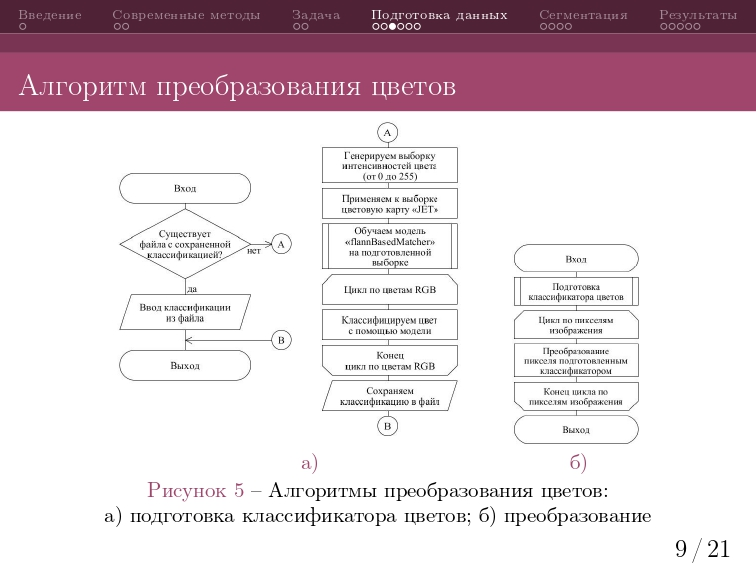
\includegraphics[width = 0.8\textwidth]{image/процентовка1_page-0009}	
		\caption{Страница презентации 9}
	\end{figure}
	\begin{figure}[h!]
		\centering
		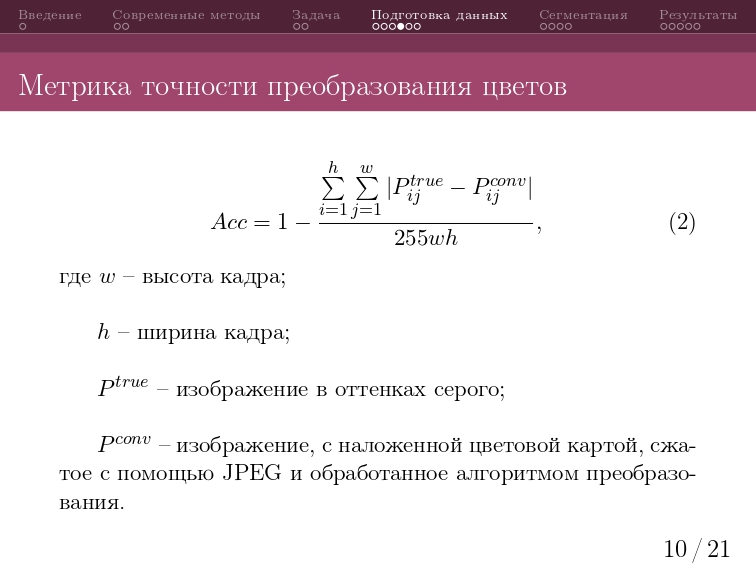
\includegraphics[width = 0.8\textwidth]{image/процентовка1_page-0010}	
		\caption{Страница презентации 10}
	\end{figure}
	\begin{figure}[h!]
		\centering
		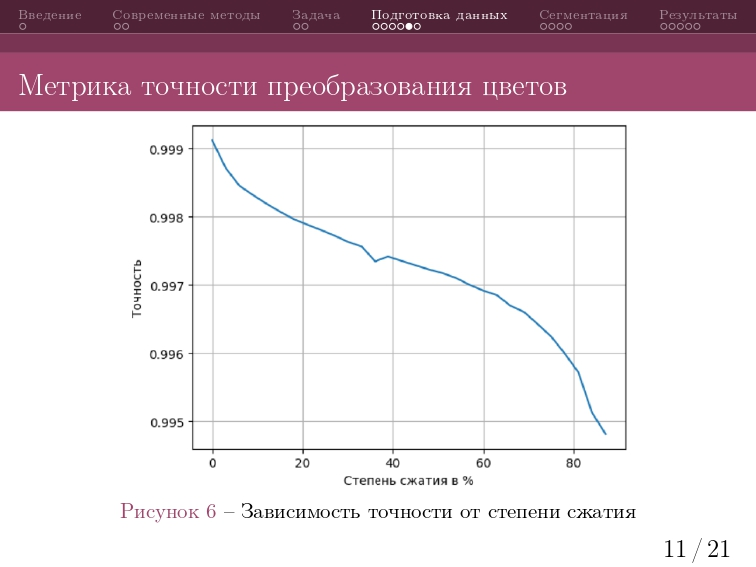
\includegraphics[width = 0.8\textwidth]{image/процентовка1_page-0011}	
		\caption{Страница презентации 11}
	\end{figure}
	\begin{figure}[h!]
		\centering
		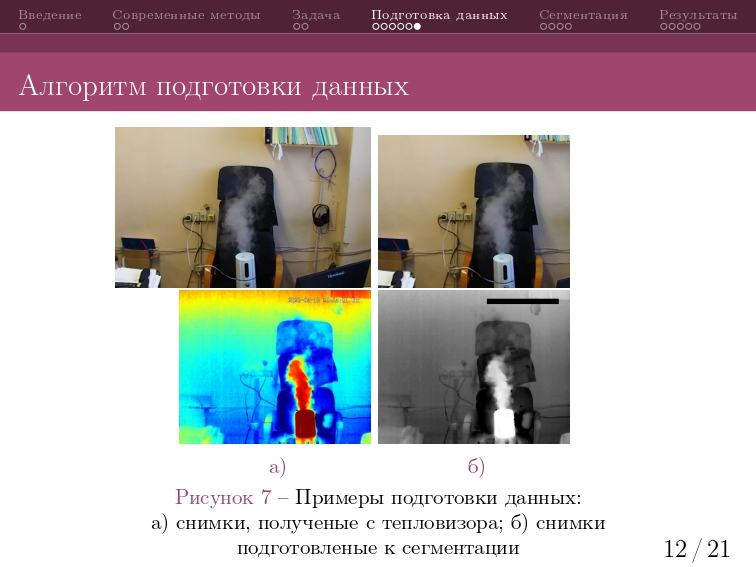
\includegraphics[width = 0.8\textwidth]{image/процентовка1_page-0012}	
		\caption{Страница презентации 12}
	\end{figure}
	\begin{figure}[h!]
		\centering
		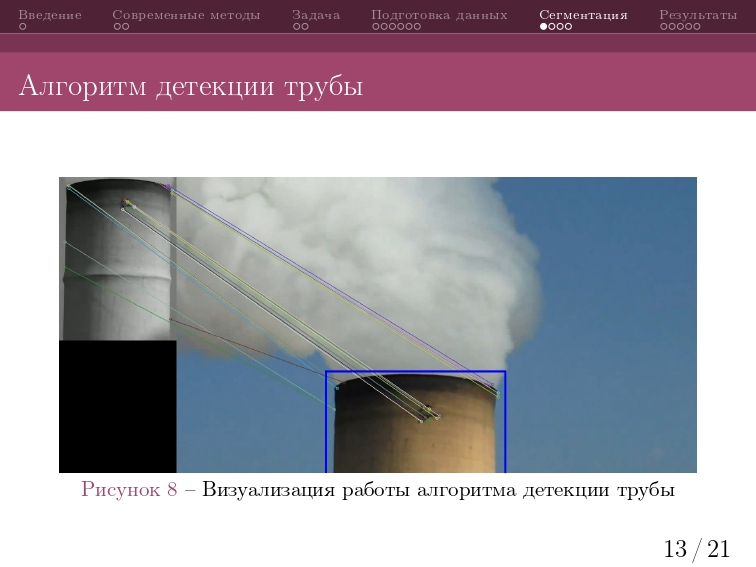
\includegraphics[width = 0.8\textwidth]{image/процентовка1_page-0013}	
		\caption{Страница презентации 13}
	\end{figure}
	\begin{figure}[h!]
		\centering
		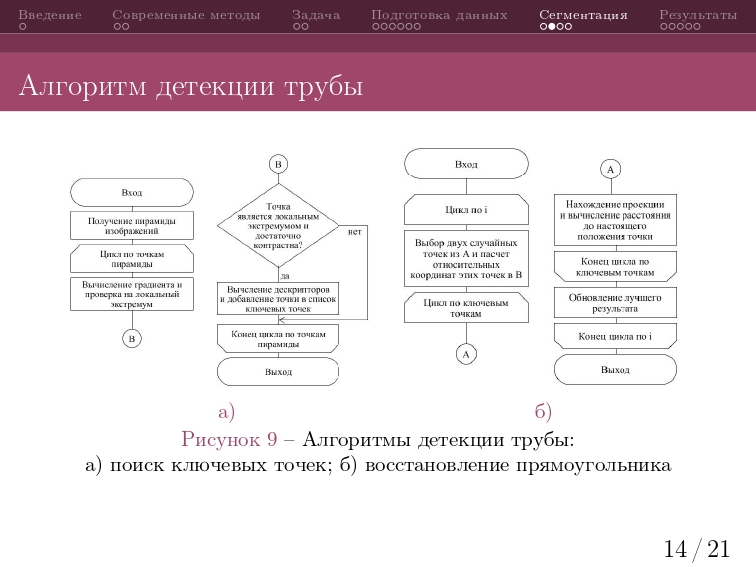
\includegraphics[width = 0.8\textwidth]{image/процентовка1_page-0014}	
		\caption{Страница презентации 14}
	\end{figure}
	\begin{figure}[h!]
		\centering
		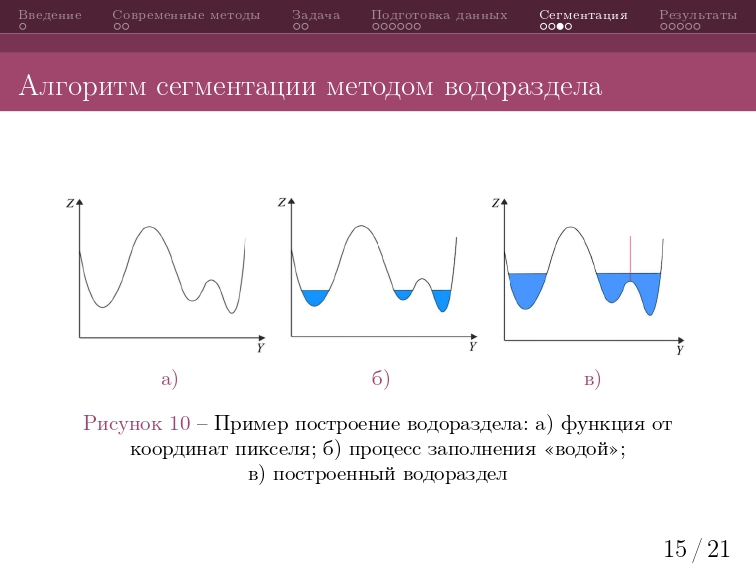
\includegraphics[width = 0.8\textwidth]{image/процентовка1_page-0015}	
		\caption{Страница презентации 15}
	\end{figure}
	\begin{figure}[h!]
		\centering
		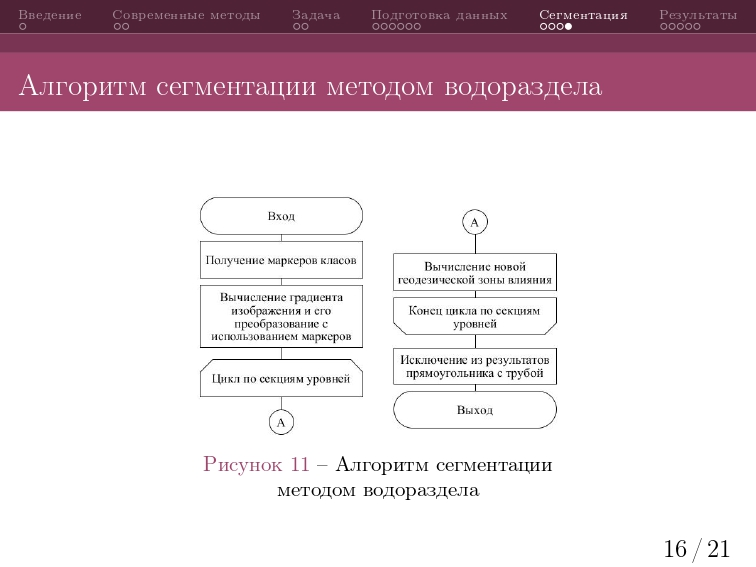
\includegraphics[width = 0.8\textwidth]{image/процентовка1_page-0016}	
		\caption{Страница презентации 16}
	\end{figure}
	\begin{figure}[h!]
		\centering
		\includegraphics[width = 0.8\textwidth]{image/процентовка1_page-0017}	
		\caption{Страница презентации 17}
	\end{figure}
	\begin{figure}[h!]
		\centering
		\includegraphics[width = 0.8\textwidth]{image/процентовка1_page-0018}	
		\caption{Страница презентации 18}
	\end{figure}
	\begin{figure}[h!]
		\centering
		\includegraphics[width = 0.8\textwidth]{image/процентовка1_page-0019}	
		\caption{Страница презентации 19}
	\end{figure}
	\begin{figure}[h!]
		\centering
		\includegraphics[width = 0.8\textwidth]{image/процентовка1_page-0020}	
		\caption{Страница презентации 20}
	\end{figure}
	\begin{figure}[h!]
		\centering
		\includegraphics[width = 0.8\textwidth]{image/процентовка1_page-0021}	
		\caption{Страница презентации 21}
	\end{figure}
\end{document}
